% figure: 777-7-13-ans-双反馈信号标注.png
% Faithful redraw of exercise 7-13, with signals defined in the solution.
% All three ideal samplers have period T and the same sampling instants.
% E = R - B2; U = E* - B1; B1 = H1 Y*; B2 = H2 Y*; Y = G U.
\documentclass[border=10pt]{standalone}
\usepackage{fontspec}
\setmainfont{Cambria}
\usepackage{unicode-math}
\setmathfont{Cambria Math}
\usepackage{tikz}
\usetikzlibrary{arrows.meta}

\definecolor{figink}{HTML}{1E2228}
\definecolor{figblue}{HTML}{1F3D7A}
\definecolor{figred}{HTML}{B23020}
\definecolor{figfill}{HTML}{E8EFF8}

\begin{document}
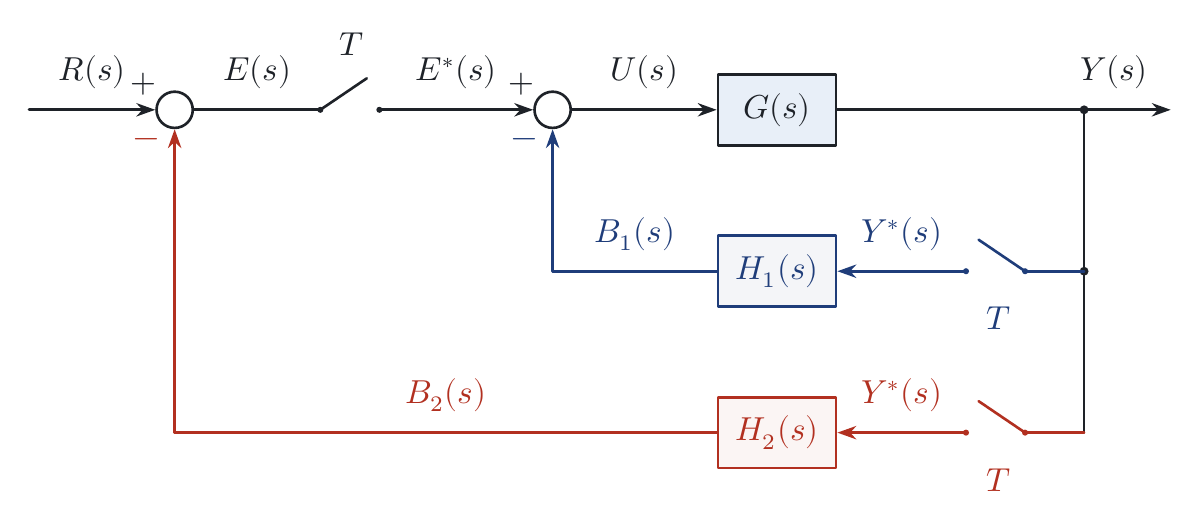
\begin{tikzpicture}[
  x=1cm,y=1cm,
  draw=figink,text=figink,
  line width=0.95pt,line cap=round,line join=round,
  >={Stealth[length=2.4mm,width=1.7mm]},
  every node/.style={font=\large},
  block/.style={draw,minimum width=1.5cm,minimum height=0.90cm,
    inner sep=3pt,fill=figfill},
  sum/.style={draw,circle,minimum size=0.46cm,inner sep=0pt,fill=white},
  sig/.style={font=\large,text=figink,inner sep=2pt,fill=white},
  sign/.style={font=\large,text=figink,inner sep=1pt,fill=white}
]

\node[sum] (outer) at (0,0) {};
\node[sum] (inner) at (4.8,0) {};
\node[block] (g) at (7.65,0) {$G(s)$};
\node[block,draw=figblue,text=figblue,fill=figblue!5]
  (h1) at (7.65,-2.05) {$H_1(s)$};
\node[block,draw=figred,text=figred,fill=figred!5]
  (h2) at (7.65,-4.10) {$H_2(s)$};

% Forward path: E is before the sampler; E* is after it.
\draw[->] (-1.85,0) -- node[sig,above=5pt] {$R(s)$} (outer.west);
\draw (outer.east) -- node[sig,above=5pt] {$E(s)$} (1.85,0);
\fill[figink] (1.85,0) circle (1.1pt);
\draw (1.85,0) -- (2.44,0.40);
\fill[figink] (2.60,0) circle (1.1pt);
\node[sig] at (2.22,0.83) {$T$};
\draw[->] (2.60,0) -- node[sig,above=5pt] {$E^{\ast}(s)$} (inner.west);
\draw[->] (inner.east) -- node[sig,above=5pt] {$U(s)$} (g.west);
\draw[->] (g.east) -- node[sig,above=5pt,pos=0.83] {$Y(s)$} (12.65,0);

% Both feedback samplers receive the same continuous output Y(s).
\fill[figink] (11.55,0) circle (1.6pt);
\draw (11.55,0) -- (11.55,-4.10);
\fill[figink] (11.55,-2.05) circle (1.6pt);

% Inner feedback: sample Y, pass through H1, subtract B1 at the inner sum.
\draw[figblue] (11.55,-2.05) -- (10.80,-2.05);
\fill[figblue] (10.80,-2.05) circle (1.1pt);
\draw[figblue] (10.80,-2.05) -- (10.21,-1.65);
\fill[figblue] (10.05,-2.05) circle (1.1pt);
\node[sig,text=figblue] at (10.43,-2.65) {$T$};
\draw[->,figblue] (10.05,-2.05)
  -- node[sig,text=figblue,above=5pt] {$Y^{\ast}(s)$} (h1.east);
\draw[figblue] (h1.west)
  -- node[sig,text=figblue,above=5pt] {$B_1(s)$} (4.8,-2.05);
\draw[->,figblue] (4.8,-2.05) -- (inner.south);

% Outer feedback: sample Y, pass through H2, subtract B2 at the outer sum.
\draw[figred] (11.55,-4.10) -- (10.80,-4.10);
\fill[figred] (10.80,-4.10) circle (1.1pt);
\draw[figred] (10.80,-4.10) -- (10.21,-3.70);
\fill[figred] (10.05,-4.10) circle (1.1pt);
\node[sig,text=figred] at (10.43,-4.70) {$T$};
\draw[->,figred] (10.05,-4.10)
  -- node[sig,text=figred,above=5pt] {$Y^{\ast}(s)$} (h2.east);
\draw[figred] (h2.west)
  -- node[sig,text=figred,above=5pt] {$B_2(s)$} (0,-4.10);
\draw[->,figred] (0,-4.10) -- (outer.south);

% Signs stay outside the summing circles and clear of the signal lines.
\node[sign] at (-0.40,0.32) {$+$};
\node[sign,text=figred] at (-0.36,-0.42) {$-$};
\node[sign] at (4.40,0.32) {$+$};
\node[sign,text=figblue] at (4.44,-0.42) {$-$};

\end{tikzpicture}
\end{document}
